\documentclass[a4paper]{article}

\usepackage[czech]{babel}
\usepackage[utf8]{inputenc}
\usepackage[T1]{fontenc}
\usepackage{outlines}
\usepackage[hidelinks]{hyperref}

\usepackage[left=1.5cm, text={18cm, 26cm}, top=1.8cm]{geometry}

\usepackage{graphicx}
\usepackage{float}
\usepackage[usenames, dvipsnames]{xcolor}

\hypersetup {
    unicode = true,
    pdfauthor = {David Konečný, Martin Pech},
    pdftitle = {Simulační studie},
    pdfsubject = {IMS},
    pdfkeywords = {IMS Projekt, balistika, ShKH vz. 77 Dana},
    % pdfproducer = {},
    % pdfcreator = {pdfTeX}
}            

\newcommand{\logo} {
    
\includegraphics[scale=0.8, keepaspectratio]{fig/logo.pdf}
}

\renewcommand*{\ttdefault}{lmtt}

\pdfminorversion=7


\begin{document}

    \begin{titlepage}
        \begin{center}
            \logo
            \\\vspace{\stretch{0.382}}
            {\Huge Simulační studie}\\\medskip
            {\LARGE Implementace abstraktního modelu autobusové linky}\\\medskip
            {\large	Hromadná osobní přeprava}
            \vspace{\stretch{0.618}}
        \end{center}
        {\Large \today \hfill
        \begin{tabular}{l l}
            \textbf{Martin Pech} & \textbf{(\texttt{xpechm00})} \\
            Josef Škorpík & (\texttt{xskorp04})
        \end{tabular}}
    \end{titlepage}

    \newpage

	\section{Úvod}
    \label{sec:intro}

    Tématem tohoto projektu je implementace abstraktního modelu~\cite[snímek 10]{IMS_slides} autobusové linky.
    Projekt vznikl jako zápočtová práce do předmětu Modelování a simulace. Chování modelu bylo demonstrováno na základě existující Jihomoravské autobusové linky číslo 501. Tento model si klade za cíl najít optimální počet autobusů, které je potřeba rezerovovat pro danou linku tak, aby nedocházelo k dlouhému čekání a najít optimální jízdní řád na základě zadaných parametrů o hustotě provozu a podobně. Jelikož je tento simulační model~\cite[snímek 44]{IMS_slides} zacílen pouze na tyto konkrétní cíle, uvažuje pouze takové jevy, které přímo ovlivňují chování modelu. Tyto jevy jsou popsány v kapitole ~\ref{subsec:conceptual_model_description}).

        \subsection{Autoři a~původ faktů}
        \label{subsec:authors}

            Na implementaci projektu a~tvorbě technické zprávy spolupracovali studenti Fakulty informačních technologií Vysokého učení technického v~Brně, Martin Pech a~Josef Škorpík.
            
            Údaje o počtu zastávek, průměrné době mezi zastávkami a intervalech mezi výjezdy autobusů, které byly použity pro výchozí nastavení modelu vycházejí z veřejně přístupných jízdních řádů uveřejněných na webu Integrovaného dopravního systému Jihomoravského kraje. 
            Pravděpodobnost výskytu dopravní nehody byla spočítána na základě veřejně dostupných statistik pro rok 2020, které každoročně uveřejňuje Policie České republiky a podle informací poskytnutých Ministerstevm dopravy České republiky k říjnu roku 2020. Pro výpočet této hodnoty bylo uvažováno následujících faktů:
            \begin{outline}
            	\1 Počet platných řidičských průkazů: \textbf{6 002 348}
            	\1 Počet dopravních nehod: \textbf{94 797}
            	\2 Z toho počet dopravních nehod s jedoucím nekolejovým vozidlem: \textbf{28 333}
            \end{outline}
            
            Pro výpočet cílové pravděpodobnosti bylo dále uvažováno, že se žádná osoba neúčastnila nehody vícekrát. Výsledná pravděpodobnost se tedy rovná přibližně \textbf{1 : 212}.
            
            Výchozí údaje o dopravní zácpě byly vysledovány -> na základě aktuální uzavírky v useky blah blah a době strávené čekáním. 

        \subsection{Validace výstupů}
        \label{subsec:validation}
			
			
			
            Jelikož je tato houfnice dostupná pouze jako inventář Ministerstva obrany, není možné pro účely tohoto simulačního modelu validovat přesně to, co tento model zkoumá.
            Jelikož ale Armáda ČR používá toto vozidlo více než 40 let (a~to v mnoha různých verzích), lze za validní data považovat technické parametry vozidla, uvedené na webu Armády ČR.
            Zkombinujeme-li tato data pro účely tohoto simulačního modelu, dá se předpokládat, že jsou výstupy tohoto modelu validní.

    \section{Rozbor tématu a~použitých metod/technologií}
    \label{sec:methods}

        Samohybná kanónová houfnice Dana (dále jen \uv{houfnice Dana}) je dělostřelecká zbraň ve verzích s automatickým, nebo manuálním nabíjením. Pro účely tohoto modelu uvažujeme pouze verzi s~manuální nabíjením.
        \uv{Vyznačuje se velkým dostřelem, přesností a~rychlostí střelby. Patří do kategorie vojenská bojová vozidla.}~\cite{Houfnice}. 
        Dále se vyznačuje rychlostí jízdy až 80 km/h po zpevněném povrchu (a~to až do vzdálenosti 800 km) a~25 km/h při jízdě v terénu (do vzdálenosti 400 km). Osádku tvoří pětičlenná skupina vojáků, která tvoří jednotku.
        Při palbě s manuálním nabíjením dosahuje rychlosti střelby až dvou výstřelů za minutu. Zajímavostí je, že v případě verze s automatickým nabíjením se rychlost střelby více než zdvojnásobí až na 5 výstřelů za minutu.~\cite{Houfnice2} 

        V tomto simulačním modelu uvažujeme situaci, kdy je v základním táboře odstaven uživatelem zadaný počet houfnic Dana. Jakmile je vyhlášena bojová pohotovost a~je vytvořen požadavek na palbu, přesouvá se jedna dostupná houfnice na bojiště,
        kde po určitou dobu vykonává činnost spojenou se svým úkolem. Na bojiště se takto může přesunou 1 – N houfnic podle toho, kolik dostane základní tábor požadavků na palbu.
        V případě, že houfnice dokončí svou činnost na bojišti (uvažujeme situaci, kdy byly zničeny všechny nepřátelské cíle, nebo houfnice vystřílela veškerou munici), vrací se houfnice zpět do základního tábora, kde probíhá její příprava na další akci.
        Houfnici lze znovu použít až ve chvíli, kdy je plně přezbrojena. U~houfnice, která se nachází na bojišti, může dojít k poruše děla. V takovém případě je houfnici potřeba dostat do základního tábora, kde podstoupí opravu.
        Její místo musí nahradit jiná dostupná houfnice.  

        Houfnice nemůže fungovat bez obsluhy, tudíž je vždy potřeba příslušný počet vojáků pro její obsluhu a~případnou opravu. Pro obsluhu houfince je potřeba jedna jednotka.
        Jednotky vojáků mohou z války dezertovat (zběhnout) s výchozí pravděpodobností $0,9^5$\%, nebo s mírou, kterou zadá uživatel simulace.~\cite{Desertion}

        \subsection{Popis použitých postupů}
        \label{subsec:methods}

            Pro tvorbu základní koncepce tohoto projektu bylo využito deklarativních modelů~\cite[snímek 49]{IMS_slides}, konkrétně Petriho sítě~\cite[snímek 123]{IMS_slides} vyobrazené níže.
            Pomocí Petriho sítí byla vytvořena obslužná linka simulující chování samohybné houfnice Dana a~obsluhujících vojáků. Pro následnou tvorbu simulačního modelu (abstraktního modelu zapsaného formou programu) bylo využito jazyku C++ a~knihovny SIMLIB.
            Zde bylo nutné důkladně nastudovat vlastnosti a~chování knihovny SIMLIB, zejména pro správnou práci s modelováním náhodných procesů~\cite[snímek 72]{IMS_slides}. 

        \subsection{Popis původu použitých metod/technologií}
        \label{subsec:techology}

            Jak již bylo zmíněno, pro implementaci byl použit jazyk C++ v~kombinaci s~knihovnou SIMLIB ve verzi 3.09\footnote{\url{https://www.fit.vutbr.cz/~peringer/SIMLIB/}}. S~pomocí tohoto jazyka
            bylo přistupováno k~rozhraní knihovny SIMLIB, pomocí kterého byly vytvořeny předpisy pro všechny komponenty potřebné k~simulaci.
            Pro sestavení programu byl použit GNU Make\footnote{\url{https://www.gnu.org/software/make/}}.

    \section{Koncepce modelu}
    \label{sec:concept}

        Konceptuální model~\cite[snímek 48]{IMS_slides} je koncipován jako systém hromadné obsluhy~\cite[snímek 136]{IMS_slides}.
        Naše dva zdroje -- jednotky vojáků a~houfnice jsou vyjádřeny obslužnými linkami. Houfnice představuje obslužná linka s~kapacitou 2,
        jednotky vojáků obslužná linka s~kapacitou 3. Do modelu vstupuje ještě jeden činitel -- dezerce, míra dezerce jednoho vojáka je stanovena na 0,9\%.
        Dezertovat může pouze celá jednotka.

        \subsection{Popis konceptuálního modelu}
        \label{subsec:conceptual_model_description}

            Do modelu vstupují požadavky na palbu, které se hromadí ve frontě, pokud je k~dispozici volná houfnice a~jednotka vojáků,
            je možné houfnici dopravit ze základního tábora na bojiště, nabít ho a~vypálit, houfnice i~s~jednotkou vojáků se poté vrací zpět do základního tábora,
            kde je opět připraven, stejně jako jednotka vojáků, obsloužit další požadavek na palbu.
            Při nabíjení však může nastat porucha, v~tom případě je houfnice dopravena do základního tábora, kde proběhně její oprava,
            po dokončení opravy je houfnice i~jednotka vojáků opět připravena obsloužit další požadavek na palbu.

        \subsection{Forma konceptuálního modelu}
        \label{subsec:conceptual_model}

            Model je reprezentován Petriho sítí, která je zobrazena níže.

            \begin{figure}[H]
                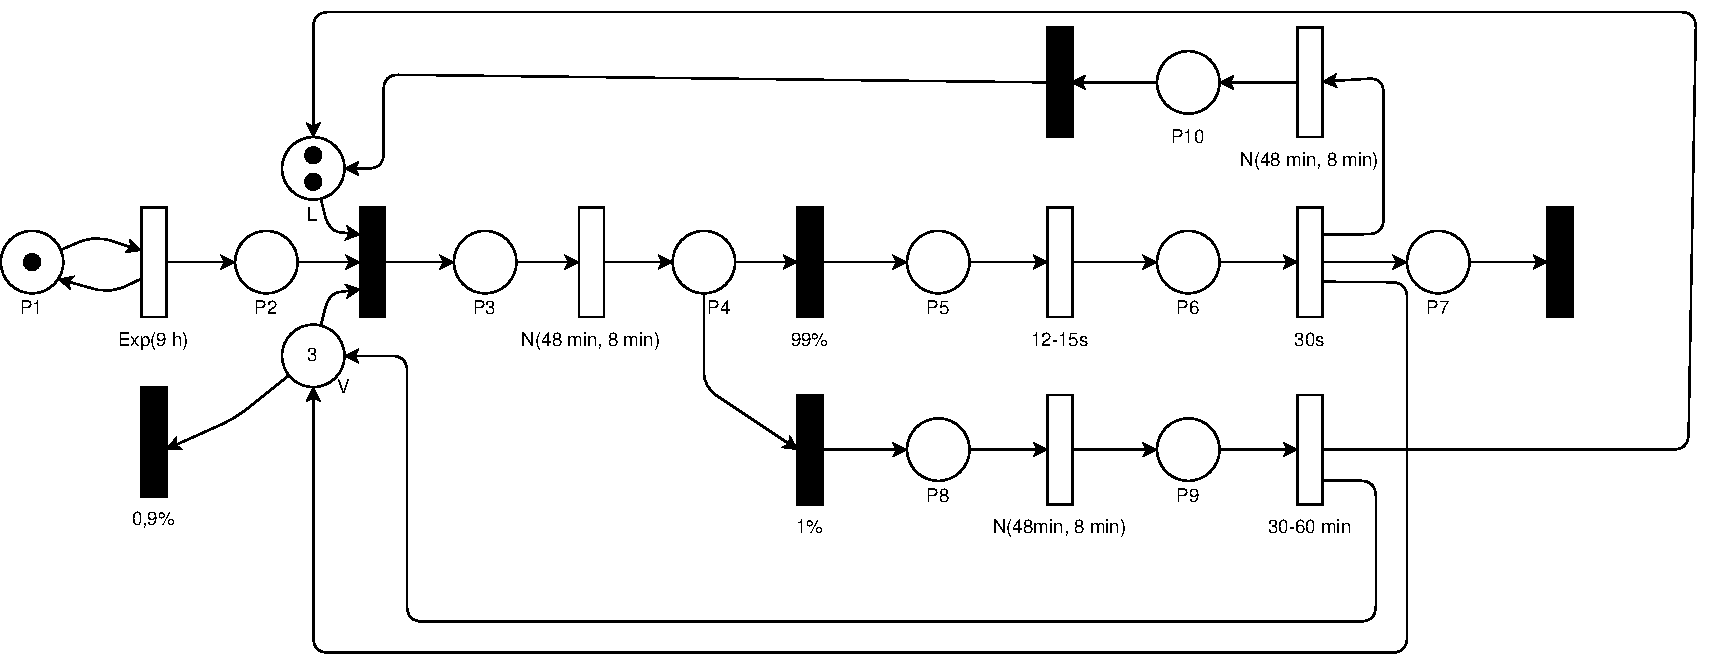
\includegraphics[scale=0.61, keepaspectratio]{fig/petri.pdf}
                \caption{Petriho síť}
                \label{fig:petri_nest}
            \end{figure}

            \begin{table}[H]
                \centering
                \begin{tabular}{ l l }
                    $P_1$ & Generování požadavků \\
                    $P_2$ & Fronta požadavků \\
                    $P_3$ & Přesun na bojiště \\
                    $P_4$ & Příprava na nabíjení \\
                    $P_5$ & Nabíjení \\
                    $P_6$ & Palba \\
                    $P_7$ & Odchod požadavků ze systému \\
                    $P_8$ & Přesun zpět do tábora (z~důvodu poruchy) \\
                    $P_9$ & Oprava houfnice \\
                    $P_{10}$ & Přesun zpět do tábora \\
                    $L$ & Linka houfnic \\
                    $V$ & Linka jednotek vojáků
                \end{tabular}
                \caption{Legenda k~Petriho síti}
                \label{tab:petri}
            \end{table}

    \section{Architektura simulačního modelu}
    \label{sec:architecture}

        Spuštěním simulačního modelu~\cite[snímek 44]{IMS_slides} se spustí simulační experiment se zadanými parametry,
        jejich zadávání je popsáno v~kapitole~\ref{subsec:start}. Během simulačního experimentu jsou vypisovány všechny změny stavu,
        výpis každé změny stavu je doprovázen modelovým časem~\cite[snímek 21]{IMS_slides}. Příkladem změny stavu může být
        přesun houfnice s~jednotkou na bojiště, palba, oprava houfnice a~další. Stavy jsou znázorněny v~Petriho síti,
        která reprezentuje konceptuální model v~kapitole~\ref{subsec:conceptual_model}.

        Pro účely simulace byla vzdálenost základního tábora od bojiště na 20 km, tomu odpovídají i~hodnoty doby přesunu,
        které vycházejí z~reálných hodnot popsaných v~kapitole~\ref{sec:methods}.

        Simulační experiment ve výchozím stavu běží tak, aby doba trvání experimentu odpovídala jednomu dni v~reálném čase~\cite[snímek 21]{IMS_slides}.
        Modelový čas~\cite[snímek 21]{IMS_slides} lze nastavit způsobem popsaným v~kapitole~\ref{subsec:start}. Jednotka modelového času je chápána jako
        minuta v~reálném čase.
        Dále zde pracujeme s~poruchovostí 1\%, která je také nastavitelná, jelikož se může měnit na základě různých vnějších vlivů, které byly v~simulaci zanedbány.

        \subsection{Mapování konceptuálního modelu do simulačního modelu}
        \label{subsec:mapping}

            Generování požadavků palby je reprezentováno třídou \texttt{Generátor}, která je implementována jako
            událost~\cite[snímek 169]{IMS_slides}. Proces přesunu na bojiště, nabíjení, palby a~návratu zpět, je 
            implementována třídou \texttt{Palba}. Dalším samostatným procesem je porucha (včetně přesunu zpět do tábora a~následné opravy),
            ta je reprezentována třídou \texttt{Porucha}. Proces dezerce jednotek vojáků je reprezentován třídou \texttt{Dezerce}.

        \subsection{Spouštění simulačního modelu}
        \label{subsec:start}

            Simulační experiment je možné spouštět s~volitelnými parametry, pokud není parametr zadán, použije se výchozí hodnota.
            
            \begin{itemize}
                \item Parametr \texttt{-t} umožňuje nastavit modelový čas, jeho výchozí hodnota je 1440, tedy 1 den.
                \item Parametr \texttt{-d} umožňuje nastavit procento dezerce (pro jednoho vojáka), výchozí hodnota je $0,9^5$\%.
                \item Parametr \texttt{-f} umožňuje nastavit intenzitu příchodu požadavků na palbu, výchozí hodnota je 540, tedy 9 hodin.
                \item Parametr \texttt{-p} umožňuje nastavit poruchovost (v~procentech), výchozí hodnota je 1\%.
            \end{itemize}

            U~všech parametrů je vyžadováno kladné číslo.

            Počet houfnic a~počet jednotek vojáků je možné měnit změnou konstanty \texttt{POCET\_RAKETOMETU} či \texttt{POCET\_VOJAKU} v~souboru \texttt{ballistics.cpp},
            poté je ještě nutné program znovu sestavit pomocí příkazu \texttt{make}.

            Program (s~výchozími hodnotami) je možné spustit příkazem \texttt{make run}.

    \section{Podstata simulačních experimentů a~jejich průběh}
    \label{sec:simulation}

        Cílem experimentů bylo pozorování chování modelu.
        Účelem bylo zjistit, na základě chování modelu, optimální vytížení obslužných linek.

        \subsection{Postup experimentování}
        \label{subsec:experiments_methods}

            Samotný experiment byl vždy spuštěn se zadanými parametry, následně byly výsledky každého experimentu
            zaneseny do tabulky. Z~výstupů experimentu byl poté vyvozen závěr.

        \subsection{Experimenty}
        \label{subsec:experiments}

            Každý experiment má svůj cíl, závěr a~nachází se u~něj výpis jeho výsledků.

            \subsubsection{Experiment 1}
            \label{subsubsec:experiment1}

                Cílem tohoto experimentu je ověření funkčnosti modelu, jsou použity výchozí hodnoty, tedy intenzita požadavků s~časem
                9 hodin (540 minut) a~dobra trvání experimentu 1 den (1440 minut).

                \begin{table}[H]
                    \centering
                    \begin{tabular}{ | c | c | c | c | c | }
                        \hline
                        Intenzita požadavků [min] & Celkový čas [min] & Bez čekání & S~čekáním & Celkem \\
                        \hline
                        \hline
                        540 & 1440 & 5 & 0 & 5 \\
                        \hline
                    \end{tabular}
                    \caption{Výsledky experimentu 1}
                    \label{tab:experiment1}
                \end{table}

                Z~výsledků experimentu vidíme, že všechny požadavky byly obslouženy, dokonce bez čekání.
                Nabízí se zde možnost existence rezervy, tzn. že systém by mohl zpracovávat více požadavků bez čekání.

            \subsubsection{Experiment 2}
            \label{subsubsec:experiment2}

                V~tomto experimentu vyzkoušíme, jak se chová systém při vyšším vytížení, intenzita požadavků byla nastavena na 30 minut.

                \begin{table}[H]
                    \centering
                    \begin{tabular}{ | c | c | c | c | c | }
                        \hline
                        Intenzita požadavků [min] & Celkový čas [min] & Bez čekání & S~čekáním & Celkem \\
                        \hline
                        \hline
                        30 & 1440 & 2 & 52 & 54 \\
                        \hline
                    \end{tabular}
                    \caption{Výsledky experimentu 2}
                    \label{tab:experiment2}
                \end{table}

                Z~tabulky~\ref{tab:experiment2} vidíme, že drtivá většina požadavků musela na svoji obsluhu čekat,
                systém byl tedy vytížen poměrně hodně.

            \subsubsection{Experiment 3}
            \label{subsubsec:experiment3}

                V~tomto experimentu si klademe za cíl najít optimální hodnotu intenzity požadavků, při které systém ještě zpracovává požadavky bez čekání.
                Postupným experimentování byla získána hodnota intenzity požadavků 130 minut.

                \begin{table}[H]
                    \centering
                    \begin{tabular}{ | c | c | c | c | c | }
                        \hline
                        Intenzita požadavků [min] & Celkový čas [min] & Bez čekání & S~čekáním & Celkem \\
                        \hline
                        \hline
                        130 & 1440 & 0 & 8 & 8 \\
                        \hline
                    \end{tabular}
                    \caption{Výsledky experimentu 3}
                    \label{tab:experiment3}
                \end{table}

                Zde vidíme, že systém zpracoval více požadavků než v~experimentu 1 v~kapitole~\ref{subsubsec:experiment1}, zároveň však byly stále všechny požadavky
                obslouženy bez čekání.

            \subsubsection{Experiment 4}
            \label{subsubsec:experiment4}

                V~tomto experimentu budeme vycházet z~hodnot a~výsledků experimentu 3 v~kapitole~\ref{subsubsec:experiment3} a~vyzkoušíme,
                zda jsou dobře využitelné i~v~delším časovém intervalu, v~tomto případě 7 dní (10080 minut).

                \begin{table}[H]
                    \centering
                    \begin{tabular}{ | c | c | c | c | c | }
                        \hline
                        Intenzita požadavků [min] & Celkový čas [min] & Bez čekání & S~čekáním & Celkem \\
                        \hline
                        \hline
                        130 & 10080 & 65 & 12 & 77 \\
                        \hline
                    \end{tabular}
                    \caption{Výsledky experimentu 4}
                    \label{tab:experiment4}
                \end{table}

                Z~výsledků je patrné, že počet požadavků, které musely na svoji obsluhu čekat, narostl,
                stále však byla většina požadavků obsloužena bez čekání.

            \subsubsection{Experiment 5}
            \label{subsubsec:experiment5}

                Cílem posledního experimentu bylo nalezení optimální hodnoty intenzity požadavků, při které systém ještě zpracovává požadavky bez čekání
                podobně jako v~experimentu 3 v~kapitole~\ref{subsubsec:experiment3}. Nalezená hodnota se nachází níže v~tabulce~\ref{tab:experiment5}.
    
                \begin{table}[H]
                    \centering
                    \begin{tabular}{ | c | c | c | c | c | }
                        \hline
                        Intenzita požadavků [min] & Celkový čas [min] & Bez čekání & S~čekáním & Celkem \\
                        \hline
                        \hline
                        260 & 10080 & 37 & 0 & 37 \\
                        \hline
                    \end{tabular}
                    \caption{Výsledky experimentu 5}
                    \label{tab:experiment5}
                \end{table}

                Vidíme, že žádný z~požadavků na svoje obsloužení nečekal, na rozdíl od experimentu 4 v~kapitole~\ref{subsubsec:experiment4} se však snížil počet všech obsloužených požadavků.
                Jelikož experiment probíhal v~intervalu jednoho týdne, na nižší počet všech obsloužených požadavků měla vliv i~poruchovost a~dezerce.

        \subsection{Závěry experimentů}
        \label{subsec:experiments_summary}

            Bylo provedeno 5 experimentů s~různými parametry. V~prvním experimentu jsme ověřili funkčnost modelu. V~dalších experimentech jsme nalezli
            časovou hodnotu intenzity požadavků, tak aby bylo vytížení obslužných linek optimální -- žádný požadavek nemusel na svoje obsloužení čekat.
            Při experimentování s~větším časovým intervalem jsme zjistili, že při optimálním vytížení obslužných linek
            může být celkový počet obsloužených požadavků nižší než počet obsloužených požadavků bez čekání při neoptimálním vytížení
            obslužných linek. Může být tedy výhodné spokojit se s~určitým počtem požadavků, které budou na svoji obsluhu čekat, za účelem
            vyššího počtu obsloužených požadavků bez čekání, což nám ukázal experiment 4 v~kapitole~\ref{subsubsec:experiment4}.
            
            Experimenty lze považovat s~dostatečnou věrohodností za správný zdroj informací, protože jich bylo provedeno několik a~vychází z~reálných dat.

    \section{Shrnutí simulačních experimentů a~závěr}
    \label{sec:summary}

        V~rámci simulačních experimentů jsme ověřili funkčnost modelu a~jeho vztah mezi simulací a~matematickými výpočty. Studií provedenou na modelu, bylo zjištěno,
        že systém vyžaduje pro optimální využití obslužných linek vhodně zvolenou intenzitu požadavků palby.
        Vhodná intenzita se liší pro časový interval, ve kterém experiment probíhal.

        V~rámci projektu vznikl nástroj, který vychází z~reálných dat dostupných na webových stránkách Armády České republiky a~Ministerstva obrany České republiky.
        Nástroj byl implementovaný v~jazyce C++ za použití knihovny SIMLIB a~umožňuje spouštět simulační experimenty
        s~různými parametry. Výstupem jsou hodnoty obsloužených požadavků a~informace zatížení obslužných linek.

    \newpage

    \renewcommand{\refname}{Použitá literatura}
    \bibliographystyle{czechiso}
    \bibliography{documentation}

\end{document}
